\documentclass[12pt,]{article}
\usepackage[T1]{fontenc}
\usepackage{lmodern}
\usepackage{amssymb,amsmath}
\usepackage{ifxetex,ifluatex}
\usepackage{fixltx2e} % provides \textsubscript
% use upquote if available, for straight quotes in verbatim environments
\IfFileExists{upquote.sty}{\usepackage{upquote}}{}
\ifnum 0\ifxetex 1\fi\ifluatex 1\fi=0 % if pdftex
  \usepackage[utf8]{inputenc}
\else % if luatex or xelatex
  \ifxetex
    \usepackage{mathspec}
    \usepackage{xltxtra,xunicode}
  \else
    \usepackage{fontspec}
  \fi
  \defaultfontfeatures{Mapping=tex-text,Scale=MatchLowercase}
  \newcommand{\euro}{€}
    \setmainfont{times}
\fi
% use microtype if available
\IfFileExists{microtype.sty}{\usepackage{microtype}}{}
\usepackage[margin=1in]{geometry}
\usepackage{graphicx}
% Redefine \includegraphics so that, unless explicit options are
% given, the image width will not exceed the width of the page.
% Images get their normal width if they fit onto the page, but
% are scaled down if they would overflow the margins.
\makeatletter
\def\ScaleIfNeeded{%
  \ifdim\Gin@nat@width>\linewidth
    \linewidth
  \else
    \Gin@nat@width
  \fi
}
\makeatother
\let\Oldincludegraphics\includegraphics
{%
 \catcode`\@=11\relax%
 \gdef\includegraphics{\@ifnextchar[{\Oldincludegraphics}{\Oldincludegraphics[width=\ScaleIfNeeded]}}%
}%
\ifxetex
  \usepackage[setpagesize=false, % page size defined by xetex
              unicode=false, % unicode breaks when used with xetex
              xetex]{hyperref}
\else
  \usepackage[unicode=true]{hyperref}
\fi
\hypersetup{breaklinks=true,
            bookmarks=true,
            pdfauthor={},
            pdftitle={},
            colorlinks=true,
            citecolor=blue,
            urlcolor=blue,
            linkcolor=magenta,
            pdfborder={0 0 0}}
\urlstyle{same}  % don't use monospace font for urls
\setlength{\parindent}{0pt}
\setlength{\parskip}{6pt plus 2pt minus 1pt}
\setlength{\emergencystretch}{3em}  % prevent overfull lines
\setcounter{secnumdepth}{0}

\author{}
\date{}
\usepackage{lineno}
\linenumbers
\usepackage{setspace}
\doublespacing

\begin{document}

\normalsize


\section{Do we need detailed demographic data to forecast population
responses to climate
change?}\label{do-we-need-detailed-demographic-data-to-forecast-population-responses-to-climate-change}

\subsubsection{Andrew T. Tredennick and Peter B.
Adler}\label{andrew-t.-tredennick-and-peter-b.-adler}

\emph{Andrew T. Tredennick
(\href{mailto:atredenn@gmail.com}{\href{mailto:atredenn@gmail.com}{atredenn@gmail.com}}),
Department of Wildland Resources and the Ecology Center, Utah State
University, Logan, UT}

\emph{Peter B. Adler, Department of Wildland Resources and the Ecology
Center, Utah State University, Logan, UT}

\subsection{Abstract}\label{abstract}

\emph{Keywords}: forecasting, climate change, grassland, integral
projection model

\subsection{Introduction}\label{introduction}

Population models are important tools for predicting the impacts of
environmental change on species. But reconciling the scales at which
population models are parameterized and the scales at which
environmental changes play out remains a challenge (Clark et al. 2010,
2012, Freckleton et al. 2011, Queenborough et al. 2011). The major
hurdle is that most population models, at least for plant species, are
built using data from small, localized plots because parameterizing
traditional population models requires tracking the fates of
individuals. These models are difficult to scale up from the micro to
meso-scales because the fitted parameters do not fully represent the
spatial variation present at scales beyond that at which the data are
collected (Sæther et al. 2007). At the same time, most demographic data
is collected over short time spans. For example, the most common study
duration in the COMPADRE matrix population model database is 4 years and
only a few exceed 10 years (Salguero-Gómez et al. 2015). The constrained
spatio-temporal extent of most demographic datasets reflects the
difficulty of collecting such data, but those constraints limit our
ability to extrapolate population models. Thus, our ability to use
population models to predict the consequences of climate change is
limited when we rely on individual-level data.

Aggregate measures of individual plant performance, such as those
typically collected as part of large-scale census efforts, offer an
alternative to detailed demographic data for modeling populations (Clark
and Bjørnstad 2004, Freckleton et al. 2011). Such population-level data
will never match the precision of individual-level data, but it is more
feasible to attain a broad coverage sample when collecting coarse-scale
data. This presents a difficult trade-off: on the one hand,
individual-level data leads to more reliable models; on the other hand,
population-level data leads to models that will produce less precise
predictions but can be applied over greater spatial and temporal
extents. An open question is how well models based on population-level
data compare to models based on individual-level data.

To date, relatively few studies have tried to model populations based on
data other than detailed individual-level data. An important exception
is an effort by Taylor and Hastings (2004) to model the population
growth rate of an invasive species to investigate the best strategies
for invasion control. They used a ``density-structured'' model where the
state variable is a discrete density state rather than a continuous
density measure. Building on this work, Freckleton et al. (2011) showed
that density-structured models compare well to continuous models in
theory, and Queenborough et al. (2011) showed the application of such
methods in a study on arable weeds. In particular, Queenborough et al.
(2011) provide empirical evidence that density-structured models are
capable of reproducing population dynamics, even if some precision is
lost when compared to fully continuous models. Thus, population models
based on coarse, population-level data show promise for producing
ecological forecasts at landscape and regional scales (Queenborough et
al. 2011). However, none of these models included environmental
covariates.

Basing population models on aggregated individual-level data in a
climate change context is hampered by the fact that it is individuals
that respond to climate, not populations (Clark et al. 2012). This fact
puts us in uneasy proximity to an ``ecological fallacy'' where one
deduces inference on the individual from statistical inference on the
group (Piantadosi et al. 1988). For example, individual plants may
respond positively to precipitation but a negative trend is observed at
the population level due to increased competition among plants as they
grow larger and consume more resources. Thus, it is important to ask the
question: Can aggregated data be used to detect climate signals of the
same sign and magnitude as individual-level data? If not, then building
population models with climate covariates on aggregated data will lead
to incorrect forecasts.

Here, we test the assumption that statistical and population models
based on aggregated data can detect climate signals as wells as models
based on individual-level data. We use a unique demographic dataset that
tracks the fates of individual plants from four species over 14 years to
build single-species population models, since those are often used tools
for ecological forecasts and climate vulnerability assessments. We first
fit population models with interannual variation in vital rates
explained, in part, by climate covariates. We then perturb the climate
covariates to test the sensitivities of species to climate change. By
doing these analyses using both individual and aggregated forms of the
same data, we provide a rigorous test of our hypothesis. We find
that\ldots{}

\subsection{Materials and Methods}\label{materials-and-methods}

\subsubsection{Study site and data}\label{study-site-and-data}

Our demographic data comes from the Fort Keogh Livestock and Range
Research Laboratory in eastern Montana's northern mixed prairie near
Miles City, Montana, USA ($46^{\circ}$ 19' N, $105^{\circ}$ 48' W). The
dataset is freely available on Ecological Archives (Anderson et al.
2011), and interested readers should refer to the metadata therein for a
complete description. The site is about 800 m above sea level and mean
annual precipitation (1878-2009) is 334 mm, with most annual
precipitation falling from April through September. The site is grass
dominated and, for the purposes of our study, we focus on the four most
abundant graminoid species: \emph{Bouteloua gracilis} (BOGR),
\emph{Hesperostipa comata} (HECO), \emph{Pascopyrum smithii} (PASM), and
\emph{Poa secunda} (POSE).

From 1932 to 1945 individual plants were identified and mapped annually
in 44 1-$\text{m}^2$ quadrats using a pantograph. The quadrats were
distributed in six pastures, each assigned a grazing treatment of light
(1.24 ha/animal unit month), moderate (0.92 ha/aum), and heavy (0.76
ha/aum) stocking rates (two pastures per treatment). In this analysis we
account for potential differences among the grazing treatments, but do
not focus on grazing$\times$climate interactions. The annual maps of the
quadrats were digitized and the fates of individual plants tracked and
extracted using a computer program. Daily climate data, which we
aggregated into climate variables of interest, are available for the
duration of the data collection period (1932 - 1945) from the Miles City
airport, Wiley Field, 9 km from the study site.

In this paper, we model populations based on two levels of data:
individual and quadrat. The individual data is the ``raw'' data. For the
quadrat level we data we simply sum individual areal cover for each
quadrat by species. This is equivalent to a perfect census of quadrat
percent cover, so we do not need to consider measurement error. Based on
these two datasets we can compare population models built using
individual level data and aggregated quadrat level data.

\subsubsection{Stastical models of vital
rates}\label{stastical-models-of-vital-rates}

At both levels of inference (individual and quadrat), the building
blocks of our population models are vital rate regressions. For
individual level data we fit models for survival, growth, and
recruitment of new individuals for each species. At the quadrat level we
fit a single regression model for population growth. We describe the
statistical models separately since fitting the models required
different approaches. All models contain five climate covariate that we
chose \emph{a priori}: ``water year'' precipitation at \emph{t}-1
(lagppt); fall through spring precipitation at \emph{t}-1 and \emph{t}-2
(ppt1 and ppt2, respectively) and mean spring temperature at \emph{t}-1
and \emph{t}-2 (TmeanSpr1 and TmeanSpr2, respectively), where \emph{t}
is the observation year.

We fit all models using a hierarchical Bayesian approach, which we
describe in more detail below. However, for each vital rate statistical
model we also define the likelihood model we use. For the likelihood
models, \textbf{Y} is always the relevant vector of observations (e.g.,
whether a genet survived {[}1{]} or not {[}0{]} from year $t$ to $t+1$).

\paragraph{Vital rate models at the individual
level}\label{vital-rate-models-at-the-individual-level}

We used logistic regression to model survival probability ($S$) of genet
$i$ from species $j$ in quadrat group $Q$ from time $t$ to $t+1$:

\begin{align}
\text{logit}(S_{ijQ,t}) &= \gamma^{S}_{j,t} + \phi^{S}_{jQ} + \beta^{S}_{j,t}x_{ij,t} + \omega^{S}_{j}w_{ij,t} + \theta^{S}_{jk}C_{k,t} + \varepsilon^{S}_{t} \\
Y^{S}_{ijQ,t} &\sim \text{Bernoulli}(S_{ijQ,t})
\end{align}

where $x_{ij,t}$ is the log of genet size, $\gamma^{S}_{j,t}$ is a
year-specific intercept, $\beta^{S}_{j,t}$ is the year-specific slope
parameter for size, $\phi^{S}_{jQ}$ is the random effect of quadrat
group location, and $\theta^{S}_{k}$ is the fixed parameter for the
effect of the $k$th climate covariate at time $t$ ($C_{k,t}$). We
include density-dependence by estimating the effect of crowding on the
focal individual by other individuals of the same species. $\omega$ is
the effect of crowding and $w_{t,Q}$ is the crowding experienced by the
focal individual at time $t$ in quadrat group $Q$.

We modeled growth as Gaussian process describing genet size at time
$t+1$ as a function of size at $t$ and climate covariates:

\begin{align}
x_{ijQ,t+1} &= \gamma^{G}_{j,t} + \phi^{G}_{jQ} + \beta^{G}_{j,t}x_{ij,t} + \omega^{G}_{j}w_{ij,t} + \theta^{G}_{jk}C_{k,t} \\
Y^{G}_{ijQ,t} &\sim \text{Normal}(x_{ijQ,t+1}, \sigma_{j})
\end{align}

where $x$ is log genet size and all other parameters are as described
for the survival regression.

Our data allows us to track new recruits, but we cannot assign a
specific parent to new genets. So, for recruitment, we work at the
quadrat level and model the number of new individuals of species $j$ in
quadrat $q$ recruiting at time $t+1$ as a function of quadrat
``effective cover'' ($A'$) in the previous year ($t$). Effective cover
is a mixture of observed cover ($A$) in the focal quadrat ($q$) and the
mean cover across the entire group ($\bar{A}$) of $Q$ quadrats in which
$q$ is located:

\begin{equation}
A'_{jq,t} = p_{j}A_{jq,t} + (1-p_{j})\bar{A}_{jQ,t}
\end{equation}

where $p$ is a mixing fraction between 0 and 1 that is estimated within
the model.

We assume the number of individuals, $Y^{R}$, recruiting at time $t+1$
follows a negative binomial distribution:

\begin{equation}
Y^{R}_{jq,t+1} \sim \text{NegBin}(\lambda_{jq,t+1},\zeta)
\end{equation}

where $\lambda$ is the mean intensity and $\zeta$ is the size parameter.
We define $\lambda$ as:

\begin{equation}
\lambda_{jq,t+1} = A'_{jq,t}e^{(\gamma^{R}_{j,t} + \phi^{R}_{jQ} + \theta^{R}_{jk}C_{k,t} + \omega^{R}\sqrt{A'_{q,t}})}
\end{equation}

where $A'$ is effective cover ($\text{cm}^2$) of species $j$ in quadrat
$q$ and all other terms are as in the survival and growth regressions.

\paragraph{Population model at the quadrat
level}\label{population-model-at-the-quadrat-level}

The statistical approach used to model vital rates using aggregated data
depends on the type of data collected. In our case, and as is often the
case with census data, we have percent cover data (which can easily be
transformed to proportion data, of course). We first considered fitting
three vital rate models analagous to those we fit at the individual
level: one for probability of extirpation within a quadrat (analagous to
survival), one for cover change within a quadrat (analagous to growth),
and one for probability of colonization within a quadrat (analagous to
recruitment). However, within-quadrat extirpation and colonization
events were rare in our time series ($N=9$ and $N=10$, respectively
across all species). Given the broad spatial distribution of the
quadrats we are studying, it is safe to assume that these events are in
fact rare enough to be ignored for our purposes. So we constrained our
statistical modeling of vital rates at the population level to change in
percent cover within quadrats. For the remaining discussion of
statistical modeling we refer to proportion data, which is simply
percent data divided by 100.

An obvious choice for fitting a linear model to proportion data is beta
regression because the support of the beta distribution is {[}0,1{]},
not including true zeros or ones. However, when we used fitted model
parameters from a beta regression in a quadrat-based population model
the simulated population tended toward 100\% cover for all species. We
therefore chose a more constrained modeling approach based on a
truncated log-normal likelihood. The model for quadrat cover change
($G$) from time $t$ to $t+1$ is

\begin{align}
x_{jq,t+1} &= \gamma^{G}_{j,t} + \phi^{G}_{jQ} + \beta^{G}_{j,t}x_{jq,t} + \theta^{S}_{jk}C_{k,t} \\
Y^{G}_{jq,t+1} &\sim \text{LogNormal}(x_{jq,t+1}, \tau{j}) T[0,1]
\end{align}

where $x_{jq,t}$ is the log of species' $j$ proportional cover in
quadrat $q$ at time $t$ and all other parameters are as in the
individual-level growth model (Eq. \#). The log normal likelihood
includes a truncation ($T${[}0,1{]}) to ensure that predicted values do
not exceed 100\% cover.

\subsubsection{Model fitting}\label{model-fitting}

Our Bayesian approach to fitting the vital rate models required choosing
appropriate priors for unknown parameters and deciding which, if any, of
those priors should be hierarchical. We decided to fit models where all
terms except climate covariates were fit by species, while the climate
covariates were fit hierarchically with species-specific coefficients
drawn from a shared `global' coefficient distribution. We did so for two
reasons: (1) the four focal species are all perennial grasses that we
expect to respond similarly to climate covariates, and (2) convergence
of climate effects at the quadrat level was much easier to achieve when
we modeled these terms hierarchically, allowing them to ``share''
statistical strength via partial pooling (Gelman and Hill 2007). So,
climate effects were modeled as:

\begin{align}
\theta_{jk} &\sim \text{Normal}(\bar{\theta_{k}}, \sigma_{k})
\end{align}

where $\bar{\theta_{k}}$ is the interspecific effect of the $k$th
climate covariate.

We used uninformative priors for all unknown parameters, specifically:

\begin{align}
\boldsymbol{\gamma, \beta, \bar{\theta}} &\sim \text{Normal}(0, 1e^{-6}) \\
\boldsymbol{\phi} &\sim \text{Normal}(0, \boldsymbol{\sigma_{\phi}}) \\
\boldsymbol{\sigma_{\phi}} &\sim e^{(\text{Gamma}(2, 0.5))} \\
\boldsymbol{\sigma_{\theta}, \sigma_{\gamma}, \sigma_{\beta}, \tau, \zeta} &\sim \text{Gamma}(0.001, 0.001)
\end{align}

All of our analyses (model fitting and simulating) were conducted in R
(Team 2013). We used the MCMC sampler in JAGS (Plummer 2003) to estimate
the posterior distributions of model parameters and the package `rjags'
to connect R to JAGS. We obtained posterior distributions for all model
parameters from three parallel MCMC chains run for 50,000 iterations,
thinned by 50, after discarding an initial 50,000 iterations. We
assessed convergence visually and using the Gelman and Rubin (1992)
diagnostic in the R package `coda' (Plummer et al. 2006). Scale
reduction factors for all parameters were less than 1.01, indicating
convergence. For the purposes of introducing stochasticity in our
population models, we saved the final 1,000 iterations from each of the
three MCMC chains for all parameters to be used as randomly drawn values
during population simulation.

\subsubsection{Population models}\label{population-models}

With the posterior distribution of the vital rate statistical models in
hand, it is straightforward to simulate the population models. We used
an Integral Projection Model (IPM) to model populations based on
individual level data and an quadrat based version of an
individually-based model (Quadrat-Based Model, QBM) to model populations
based on quadrat level data. Both models take the general form:

\begin{equation}
N_{t+1} = S \times G + R.
\end{equation}

So, at each time step in a simulation, we use the survival regression to
determine if each genet lives or not (if each quadrat remains occupied
or not), the growth regression to determine size changes of surviving
individuals (cover change of occupied quadrats), and the recruitment
regression to determine the number of new recruits (if a quadrat is
colonized or not). We first use one-step-ahead forecasts to assess each
model's ability to reproduce observed cover changes. Then we use the
models to analyze the effect of potential climate changes on population
size over long time scales.

We used random draws from the final 1,000 iterations from each of three
MCMC chains to introduce stochasticity into our population models. At
each time step, we randomly selected climate covariates from one of the
14 observed years. Then, we drew the full parameter set (climate effects
and density-dependence fixed effects) from a randomly selected MCMC
iteration. Using this approach, rather than simply using coefficient
point estimates, ensures that relatively unimportant climate covariates
(those that broadly overlap 0) have little effect on the simulation
results. Since our focus was on the contribution of climate covariates
to population states, we set the random year effects and the random
group effects to zero.

\subsubsection{Model validation}\label{model-validation}

To test each model's ability to forecast the population state we used
leave-one-year-out cross validation. For both levels of modeling, we fit
the vital rate models using observations from all years except one, and
then used those fitted parameters in the population models to perform a
one-step-ahead forecast for the year whose observations were withheld
from model fitting. We repeated this procedure for all 13 observation
years. This model validation allowed us to compare accuracy and
precision of the two modeling approaches (individual-level versus
population-level).

\subsection{Results}\label{results}

\subsubsection{Comparison of Forecast
Models}\label{comparison-of-forecast-models}

We performed one-step-ahead forecasts to compare the two models (IPM
vs.~QBM). We did not use the random year effects for these forecasts.
Thus, beyond the effect of genet size or quadrat cover, only the climate
covariates could affect expect plant cover. The models had similar
accuracy ($\rho$, correlation between observations and mean prediction
from 100 forecasts) across all species (Table 1). However, the IPM had
significantly lower overall error (MAE, mean absolute error) for two
species (\emph{H. comita} and \emph{P. smithii}), and in no case did the
QBM significantly outperform the IPM (Table 1).

\subsubsection{Forecasting Climate Change
Impacts}\label{forecasting-climate-change-impacts}

Equilibrium cover simulated from the models was sensitive to climate
perturbations, but the IPM and QBM produced inconsistent results (Figure
3). For \emph{B. gracilis}, the IPM predicted a modest increase in cover
with a 1\% increase in the mean of precipitation or a 1\% increase in
the mean of temperature, the compounding effect of both being a 20\%
increase in cover. This reflects the relatively strong effects of
precipitation and climate on \emph{B. gracilis} genet growth and
recruitment (Figure 1). The QBM also predicted increased \emph{B.
gracilis} cover with a precipitation increase, but increasing
temperature decreased equilibrium cover (Figure 3).

The IPM and QBM produced consistent predictions for \emph{H. comita}
under increased precipitation and when both precipitation and
temperature were increased (Figure 3). However, the IPM predicted more
modest changes than the QBM, and for a temperature increase the two
models differed: the IPM predicted an increase in cover while the QBM
predicted the opposite.

\subsection{Discussion}\label{discussion}

We sought to test the assumption that the sensitivities of plant
populations to climate variables can be detected equally well using
either individual level data or population level data. This is an
important question to answer because population models are key tools for
predicting the consequences of global climate change. However, they can
be of limited use when built on data from a small subset of a population
in space or time. If population level data (i.e., some aggregated form
of individual level data) can be used to detect climate effects on
population dynamics, then we would have a cheaper and easier option for
data collection over relatively large temporal and spatial extents
(\emph{e.g.} Freckleton et al. 2011).

It is perhaps startling that two different types of models fit using the
same data produce drastically different forecasts (Figure 3).

\pagebreak{}

\subsection{Tables}\label{tables}

\begin{table}[ht]
\centering
\caption{Mean absolute error (MAE) and accuracy (Pearson's $\rho$) for one-step-ahead forecast from both model types. Forecasts were made without random year effects; only climate covariates could explain year-to-year variation. 90 Distance refers to the average distance between the upper and lower 90 percentiles of the 100 predicted values for each quadrat-year combination.} 
\begin{tabular}{llrrr}
  \hline
Species & Model & MAE & 90\% Distance & Mean Obs. Cover \\ 
  \hline
BOGR & IPM & 4.77 & 29.33 & 9.16 \\ 
  BOGR & QBM & 5.30 & 44.63 & 9.22 \\ 
  HECO & IPM & 0.60 & 2.82 & 1.22 \\ 
  HECO & QBM & 2.03 & 12.05 & 1.25 \\ 
  PASM & IPM & 0.18 & 0.49 & 0.40 \\ 
  PASM & QBM & 0.17 & 1.34 & 0.40 \\ 
  POSE & IPM & 0.78 & 2.16 & 1.23 \\ 
  POSE & QBM & 1.30 & 7.04 & 1.25 \\ 
   \hline
\end{tabular}
\end{table}

The IPM MAE is significantly lower for HECO ($p = 3.3 \times 10^{-10}$)
and POSE ($p = 0.00013$). MAEs are statisticially similar between models
for BOGR and PASM.

\pagebreak{}

\subsection{Figures}\label{figures}

\begin{figure}[htbp]
\centering
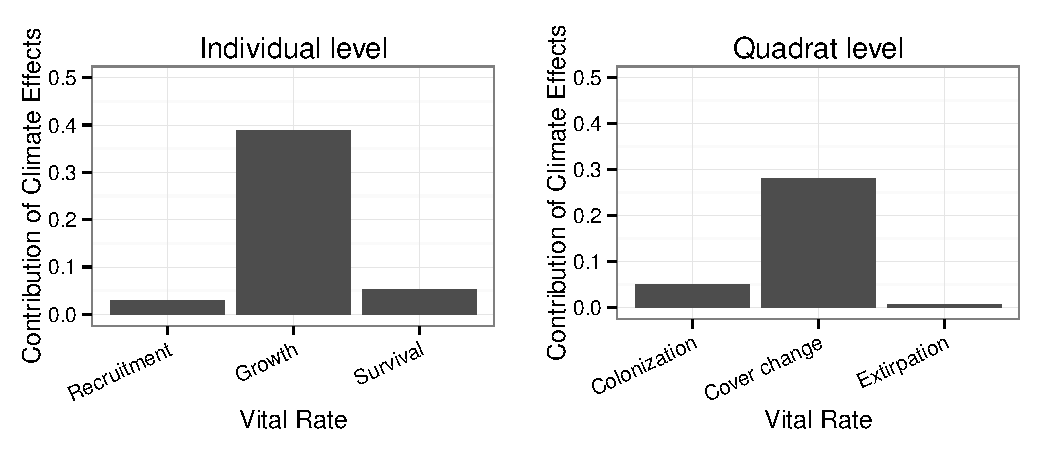
\includegraphics{components/figure/manuscript-figure_1.pdf}
\caption{Sensitivity of equilibrium cover to removal of climate effects
from each vital rate regression.}
\end{figure}

\begin{figure}[htbp]
\centering
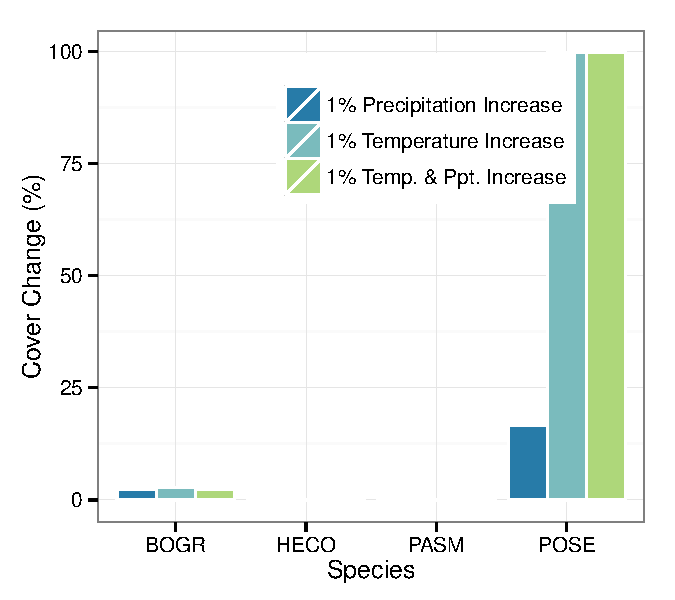
\includegraphics{components/figure/manuscript-figure_2.pdf}
\caption{Proportional change in species' mean cover caused by a 1\%
increase in observed precipitation, temperature, or both as predicted by
the individual-based IPM and the aggregate-based QBM. Note that the
change for POSE due to a precipitation increase predicted by the QBM is
almost zero and so does not show up in the figure. Labels on x-axis
refer to: `ppt' = 1\% increase in mean precipitation; `temp' = 1\%
increase in mean temperature; `ppt + temp' = 1\% increase in mean
precipitation and mean temperature.}
\end{figure}

\pagebreak{}

\subsection{References}\label{references}

Anderson, J., L. Vermeire, and P. B. Adler. 2011. Fourteen years of
mapped, permanent quadrats in a northern mixed prairie, USA. Ecology
92:1703.

Clark, J. S., and O. N. Bjørnstad. 2004. Population time series: Process
variability, observation errors, missing values, lags, and hidden
states. Ecology 85:3140--3150.

Clark, J. S., D. M. Bell, M. Kwit, A. Stine, B. Vierra, and K. Zhu.
2012. Individual-scale inference to anticipate climate-change
vulnerability of biodiversity.

Clark, J. S., D. Bell, C. Chu, B. Courbaud, M. Dietze, M. Hersh, J.
HilleRisLambers, I. Ibáñez, S. LaDeau, S. McMahon, J. Metcalf, J. Mohan,
E. Moran, L. Pangle, S. Pearson, C. Salk, Z. Shen, D. Valle, and P.
Wyckoff. 2010. High-dimensional coexistence based on individual
variation: a synthesis of evidence. Ecological Monographs 80:569--608.

Freckleton, R. P., W. J. Sutherland, A. R. Watkinson, and S. A.
Queenborough. 2011. Density-structured models for plant population
dynamics. American Naturalist 177:1--17.

Gelman, A., and J. Hill. 2007. Data analysis using regression and
multilevel/hierarchical models. Page xxii, 625p.

Gelman, A., and D. B. Rubin. 1992. Inference from Iterative Simulation
Using Multiple Sequences.

Piantadosi, S., D. P. Byar, and S. B. Green. 1988. The Ecological
Fallacy. American Journal of Epidemiology 127:893--904.

Plummer, M. 2003. JAGS: A Program for Analysis of Bayesian Graphical
Models Using Gibbs Sampling. Pages 20--22 \emph{in} Proceedings of the
3rd international workshop on distributed statistical computing (dSC
2003). march.

Plummer, M., N. Best, K. Cowles, and K. Vines. 2006. CODA: Convergence
Diagnosis and Output Analysis for MCMC. R News 6:7--11.

Queenborough, S. A., K. M. Burnet, W. J. Sutherland, A. R. Watkinson,
and R. P. Freckleton. 2011. From meso- to macroscale population
dynamics: A new density-structured approach. Methods in Ecology and
Evolution 2:289--302.

Salguero-Gómez, R., O. R. Jones, C. R. Archer, Y. M. Buckley, J.
Che-Castaldo, H. Caswell, D. Hodgson, A. Scheuerlein, D. A. Conde, E.
Brinks, H. de Buhr, C. Farack, F. Gottschalk, A. Hartmann, A. Henning,
G. Hoppe, G. Römer, J. Runge, T. Ruoff, J. Wille, S. Zeh, R. Davison, D.
Vieregg, A. Baudisch, R. Altwegg, F. Colchero, M. Dong, H. de Kroon,
J.-D. Lebreton, C. J. E. Metcalf, M. M. Neel, I. M. Parker, T. Takada,
T. Valverde, L. A. Vélez-Espino, G. M. Wardle, M. Franco, and J. W.
Vaupel. 2015. The compadrePlant Matrix Database: an open online
repository for plant demography. Journal of Ecology 103:202--218.

Sæther, B. E., S. Engen, V. Grøtan, W. Fiedler, E. Matthysen, M. E.
Visser, J. Wright, A. P. Møller, F. Adriaensen, H. {Van Balen}, D.
Balmer, M. C. Mainwaring, R. H. McCleery, M. Pampus, and W. Winkel.
2007. The extended Moran effect and large-scale synchronous fluctuations
in the size of great tit and blue tit populations. Journal of Animal
Ecology 76:315--325.

Taylor, C. M., and A. Hastings. 2004. Finding optimal control strategies
for invasive species: a density-structured model for Spartina
alterniflora. Journal of Applied Ecology 41:1049--1057.

Team, R. 2013. R Development Core Team. R: A Language and Environment
for Statistical Computing.

\end{document}
